\documentclass[a4paper, 11pt]{article}
\usepackage[english]{babel}
\usepackage[T1]{fontenc}
\usepackage[utf8]{inputenc}
\usepackage[left=1.5cm, right=2cm]{geometry}
\usepackage{fancyhdr}
\usepackage{graphicx}
\usepackage{lastpage}
\usepackage{ragged2e}
\usepackage[yyyymmdd]{datetime}

% ToC Env

\pagenumbering{arabic}
\setcounter{secnumdepth}{5}
\setcounter{tocdepth}{5}

\makeatletter
\newcommand\subsubsubsection{\@startsection{paragraph}{4}{\z@}{-2.5ex\@plus -1ex \@minus -.25ex}{1.25ex \@plus .25ex}{\normalfont\normalsize\bfseries}}
\newcommand\subsubsubsubsection{\@startsection{subparagraph}{5}{\z@}{-2.5ex\@plus -1ex \@minus -.25ex}{1.25ex \@plus .25ex}{\normalfont\normalsize\bfseries}}
\makeatother

\renewcommand{\dateseparator}{--}

% Header and Footer Definition

\pagestyle{fancy}
\renewcommand{\headrulewidth}{0.4pt}
\renewcommand{\footrulewidth}{0.4pt}
\fancyhf{}
\fancyhead[R]{\bfseries Golem Network Architecture Overview}
\fancyfoot[L]{
    \raggedright{Author: P. Rekucki, M. Rakowski \\ Company: Golem Factory}
    }
\fancyfoot[C]{
    \centering{Draft \\ Propertiary}
    }
\fancyfoot[R]{
    \raggedleft{Date: \today \\ Page: \thepage\ of \pageref{LastPage}}
    }

\begin{document}

% Title Page

\thispagestyle{empty}
\begin{flushright}
    
\includegraphics[width=100bp]{Golem.png}
\end{flushright}

\vskip4cm

\begin{flushleft}
    \huge Functional and System Architecture Document
\end{flushleft}
\hrule
\begin{flushleft}
    \LARGE Golem Network Architecture Overview
\end{flushleft}

\vskip8cm
\hrule

\begin{center}
    \Large Warsaw 2024
\end{center}

\break

% ToC

\tableofcontents

\newpage

% Sections Files

%\section{Scope}
\section{Scope}

%\section{Reference}
\section{Reference}

%\section{Definition of terms and Abbreviations}
\section{Definition of terms and Abbreviations}

\subsection{Terms}

%\subsection{Symbols}

\subsection{Abbreviations}

%\section{Framework Concept}
\section{Framework Concept}

\subsection{Introduction}

\subsection{Definitions}

\subsection{Abstract Architecture}

%\begin{figure}
%    \centering
%    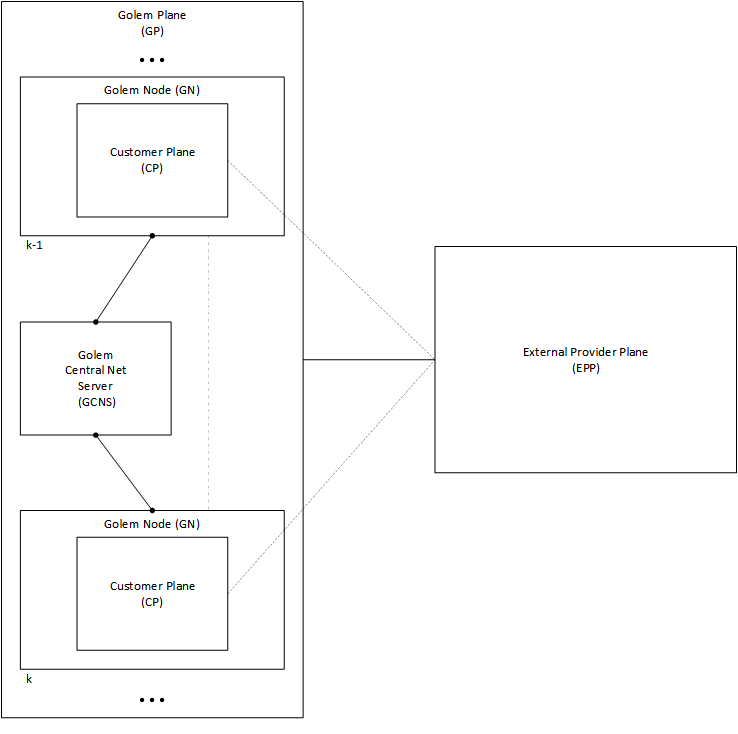
\includegraphics[width=7cm,height=7cm,angle=0]{./diag/03.AbsPlane-Diag.png}
%    \label{Plane}
%\end{figure}

%\begin{figure}
%    \centering
%    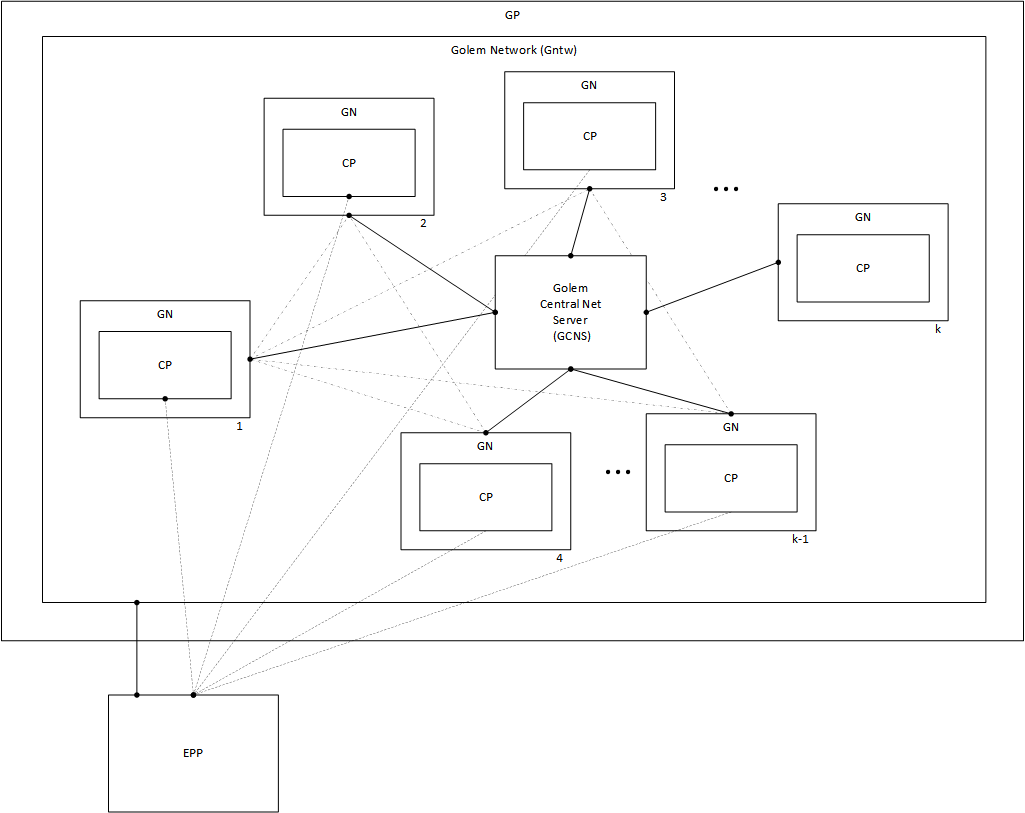
\includegraphics[width=7cm,height=7cm,angle=0]{./diag/02.AbsNtw-Diag.png}
%    \label{Plane}
%\end{figure}


\subsection{Reference Architecture}

%\section{Golem Plane}
\section{Golem Plane}

\subsection{Introduction}

\subsection{Golem Network}

\subsubsection{Introduction}

\subsubsection{Golem Node}

\subsubsubsection{Golem Agent}

\begin{enumerate}
    \item Golem Payment Gateway
    \item Golem Schedule Manager
\end{enumerate}

\subsubsubsection{Golem Orchestrator}

\begin{enumerate}
    \item Terminal User Interface
\end{enumerate}

\subsubsubsection{Golem Service Bus}

\subsubsubsubsection{Golem Net Point}

\subsubsubsubsection{Golem Market Point}

\subsubsubsubsection{Golem Activity Point}

\subsubsubsubsection{Golem Payment Point}

\subsubsubsection{Golem Abstraction Resource}

\subsubsubsubsection{Physical Resource}

\subsubsubsubsection{Golem Resource Point}

\subsubsubsection{Golem Services}

\subsubsubsubsection{Golem Net Service}

\begin{enumerate}
    \item Service Profile
    \item Service Protocol
    \item Service Interface
    \item Service Workflow
\end{enumerate}

\subsubsubsubsection{Golem Market Service}

\begin{enumerate}
    \item Service Profile
    \item Service Protocol
    \item Service Interface
    \item Service Workflow
\end{enumerate}

\subsubsubsubsection{Golem Activity Service}

\begin{enumerate}
    \item Service Profile
    \item Service Protocol
    \item Service Interface
    \item Service Workflow
\end{enumerate}

\subsubsubsubsection{Golem Payment Service}

\begin{enumerate}
    \item Service Profile
    \item Service Protocol
    \item Service Interface
    \item Service Workflow
\end{enumerate}

\subsubsubsubsection{Registry and Discovery Service}

\subsubsubsection{Golem Toolkit}

\subsubsubsubsection{Golem Net Service API}

\subsubsubsubsection{Golem Market Service API}

\subsubsubsubsection{Golem Activity Service API}

\subsubsubsubsection{Golem Payment Service API} 

\subsubsubsubsection{Golem Rest Point}

\subsubsection{Golem Central Net Server}



%\section{User Plane}
\section{User plane}

\subsection{Introduction}

\subsubsection{Ecosystem}

\subsubsubsection{SDK API}

\subsubsubsection{Examples}



%\section{External Provider Plane}
\section{External Provider Plane}

\subsection{Introduction}

\subsection{Payment Provider}

%\section{Layers}
\section{Layers}

\subsection{Platform Layer}

\subsection{APIs and Tools Layer}

\subsection{Application and Service Layer}

\end{document}